%!TEX root = paper-aaai25.tex
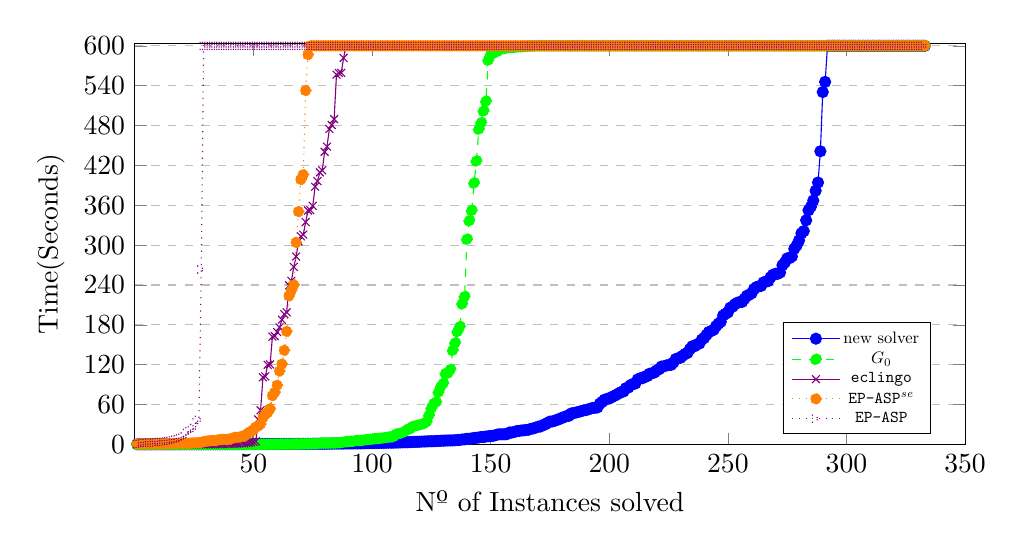
\begin{tikzpicture}
\begin{axis}[
    % title={Survival Plots for solvers},
    width=1\textwidth,
    height=0.55\textwidth,
    ylabel={Time(Seconds)},
    xlabel={Nº of Instances solved},
    ymin=0, ymax=603,
    xmin=0, xmax=350,
    ytick={0, 60, 120, 180, 240, 300, 360, 420, 480, 540, 600},
    xtick={50, 100, 150, 200, 250, 300, 350},
    legend style={
                at={(0.87,0.165)},
                anchor=center,
                legend columns=1,
                nodes={scale=0.6, transform shape},
                /tikz/every even column/.append style={column sep=0.5cm}
            },
    ymajorgrids=true,
    grid style=dashed,
]
\addplot[
    color=blue,
    mark=*,
    ]
    coordinates {
    (1,0.154922)(2,0.16203)(3,0.16743999999999998)(4,0.1717455)(5,0.1776755)(6,0.18612099999999998)(7,0.192922)(8,0.192998)(9,0.194574)(10,0.1951465)(11,0.2026765)(12,0.20275949999999998)(13,0.2119715)(14,0.2133575)(15,0.215201)(16,0.21608899999999998)(17,0.219945)(18,0.2219755)(19,0.229006)(20,0.2316645)(21,0.235128)(22,0.2425365)(23,0.2457745)(24,0.252011)(25,0.25256850000000003)(26,0.254865)(27,0.255891)(28,0.2610625)(29,0.2653535)(30,0.2660585)(31,0.26918600000000004)(32,0.30066000000000004)(33,0.30200400000000005)(34,0.3026175)(35,0.3041345)(36,0.3067565)(37,0.30746700000000005)(38,0.31862)(39,0.32464899999999997)(40,0.3256645)(41,0.3263325)(42,0.3655485)(43,0.38409899999999997)(44,0.4118465)(45,0.425622)(46,0.430578)(47,0.43336600000000003)(48,0.448606)(49,0.45592299999999997)(50,0.483968)(51,0.4881005)(52,0.4889105)(53,0.5045935)(54,0.5082450000000001)(55,0.5188925)(56,0.5458745)(57,0.560948)(58,0.5641455)(59,0.6128235)(60,0.618761)(61,0.6312105)(62,0.6723705)(63,0.6821665)(64,0.69794)(65,0.711919)(66,0.721591)(67,0.7423455)(68,0.7961125)(69,0.7980195)(70,0.808441)(71,0.836962)(72,0.839183)(73,0.933079)(74,0.942664)(75,0.9718495)(76,0.97444)(77,0.9779344999999999)(78,0.991527)(79,0.9930885)(80,1.0209700000000002)(81,1.0946449999999999)(82,1.10531)(83,1.15149)(84,1.1866349999999999)(85,1.210845)(86,1.23458)(87,1.2388750000000002)(88,1.31433)(89,1.421795)(90,1.43323)(91,1.444695)(92,1.48672)(93,1.550775)(94,1.551265)(95,1.55156)(96,1.669785)(97,1.8561999999999999)(98,1.976875)(99,2.00042)(100,2.0389049999999997)(101,2.096415)(102,2.186255)(103,2.22913)(104,2.315905)(105,2.3898650000000004)(106,2.54013)(107,2.60611)(108,2.60944)(109,2.6443899999999996)(110,2.741485)(111,2.840595)(112,3.007345)(113,3.084695)(114,3.208935)(115,3.2174750000000003)(116,3.4957000000000003)(117,3.6079600000000003)(118,3.836605)(119,3.87767)(120,4.023855)(121,4.22523)(122,4.327075)(123,4.50767)(124,4.746745)(125,4.75872)(126,4.82061)(127,5.062799999999999)(128,5.2063950000000006)(129,5.473305)(130,5.647815)(131,5.750845)(132,5.927935)(133,5.9856)(134,6.01107)(135,6.25594)(136,6.6053999999999995)(137,6.780865)(138,7.45555)(139,7.601205)(140,8.3549)(141,8.50667)(142,8.93148)(143,9.75158)(144,9.891905)(145,10.452649999999998)(146,11.08155)(147,11.118549999999999)(148,11.83055)(149,12.226099999999999)(150,12.7446)(151,12.918099999999999)(152,13.8072)(153,14.99855)(154,15.16465)(155,15.1822)(156,15.21805)(157,15.637550000000001)(158,17.998649999999998)(159,18.0412)(160,18.66775)(161,20.0746)(162,20.2927)(163,21.0214)(164,21.14295)(165,21.7038)(166,22.141350000000003)(167,23.45805)(168,24.112450000000003)(169,25.30105)(170,26.61605)(171,26.9514)(172,28.98065)(173,30.1477)(174,32.513000000000005)(175,34.3553)(176,34.602850000000004)(177,35.5378)(178,37.0947)(179,38.03035)(180,40.04715)(181,41.0664)(182,42.72505)(183,43.044)(184,46.64125)(185,47.21875)(186,47.9634)(187,48.93729999999999)(188,49.8788)(189,51.02385)(190,51.62195)(191,52.5173)(192,53.80455)(193,54.90755)(194,55.09935)(195,55.6484)(196,61.11785)(197,64.0018)(198,67.27529999999999)(199,68.43615)(200,68.97585000000001)(201,71.16885)(202,72.803)(203,74.79355)(204,76.7559)(205,78.85485)(206,79.62270000000001)(207,84.57554999999999)(208,85.4471)(209,89.161)(210,91.00555)(211,91.6671)(212,97.90975)(213,99.47255)(214,99.60055)(215,102.1345)(216,102.7355)(217,106.424)(218,107.0495)(219,108.18)(220,111.311)(221,113.22)(222,117.193)(223,117.432)(224,118.82)(225,119.5865)(226,119.605)(227,123.08000000000001)(228,128.4465)(229,129.745)(230,130.29899999999998)(231,133.5515)(232,136.2095)(233,137.7775)(234,143.461)(235,147.75549999999998)(236,147.81400000000002)(237,150.659)(238,151.886)(239,157.6635)(240,160.24149999999997)(241,164.90050000000002)(242,169.23950000000002)(243,170.856)(244,172.566)(245,177.9085)(246,181.6165)(247,184.4385)(248,194.03199999999998)(249,196.68200000000002)(250,198.5965)(251,205.7255)(252,207.32850000000002)(253,211.034)(254,213.25900000000001)(255,214.421)(256,214.50549999999998)(257,219.112)(258,223.61700000000002)(259,225.3065)(260,227.43)(261,233.64749999999998)(262,236.6765)(263,238.001)(264,238.57150000000001)(265,243.904)(266,244.97250000000003)(267,245.851)(268,251.5865)(269,255.33)(270,256.7405)(271,256.754)(272,258.7155)(273,269.6885)(274,273.637)(275,280.01)(276,280.3825)(277,282.85900000000004)(278,294.4145)(279,299.4505)(280,307.072)(281,317.73900000000003)(282,321.061)(283,337.3365)(284,352.3805)(285,357.814)(286,367.0725)(287,381.804)(288,394.17)(289,441.2795)(290,530.3815)(291,545.6645000000001)(292,600.0)(293,600.0)(294,600.0)(295,600.0)(296,600.0)(297,600.0)(298,600.0)(299,600.0)(300,600.0)(301,600.0)(302,600.0)(303,600.0)(304,600.0)(305,600.0)(306,600.0)(307,600.0)(308,600.0)(309,600.0)(310,600.0)(311,600.0)(312,600.0)(313,600.0)(314,600.0)(315,600.0)(316,600.0)(317,600.0)(318,600.0)(319,600.0)(320,600.0)(321,600.0)(322,600.0)(323,600.0)(324,600.0)(325,600.0)(326,600.0)(327,600.0)(328,600.0)(329,600.0)(330,600.0)(331,600.0)(332,600.0)(333,600.0)
};
\addlegendentry{ new solver }
% \addplot[
    color=red,
    mark=x,
    ]
    coordinates {
    (1,0.15041)(2,0.1695065)(3,0.1763245)(4,0.177056)(5,0.178106)(6,0.185884)(7,0.18772650000000002)(8,0.191318)(9,0.191753)(10,0.19479400000000002)(11,0.1952105)(12,0.20246799999999998)(13,0.202577)(14,0.2073885)(15,0.2115565)(16,0.2135805)(17,0.220354)(18,0.222414)(19,0.223356)(20,0.224848)(21,0.2252825)(22,0.22741050000000002)(23,0.22871)(24,0.239037)(25,0.24079299999999998)(26,0.2421605)(27,0.247023)(28,0.254274)(29,0.26283599999999996)(30,0.26360700000000004)(31,0.265543)(32,0.2664995)(33,0.2736325)(34,0.274786)(35,0.27784)(36,0.283919)(37,0.2869875)(38,0.290599)(39,0.292231)(40,0.297362)(41,0.318328)(42,0.3189695)(43,0.3342115)(44,0.348418)(45,0.4074955)(46,0.4137625)(47,0.429988)(48,0.43520250000000005)(49,0.463785)(50,0.466029)(51,0.47113150000000004)(52,0.47361200000000003)(53,0.4900185)(54,0.499)(55,0.5178205)(56,0.542673)(57,0.5681285)(58,0.5966265)(59,0.6486845)(60,0.6715329999999999)(61,0.688707)(62,0.7081155)(63,0.7155294999999999)(64,0.7233815)(65,0.7304685)(66,0.7634765)(67,0.7974915)(68,0.826448)(69,0.844858)(70,0.8781384999999999)(71,0.912397)(72,0.9474035000000001)(73,0.989197)(74,1.11036)(75,1.120935)(76,1.178665)(77,1.18595)(78,1.1964000000000001)(79,1.24127)(80,1.368805)(81,1.371175)(82,1.400075)(83,1.4752649999999998)(84,1.509625)(85,1.568675)(86,1.5688300000000002)(87,1.77525)(88,1.920955)(89,1.98203)(90,2.07602)(91,2.092605)(92,2.1008250000000004)(93,2.197965)(94,2.430505)(95,2.52485)(96,2.52959)(97,2.7132500000000004)(98,2.8306750000000003)(99,2.938875)(100,3.02799)(101,3.0765450000000003)(102,3.34694)(103,3.668025)(104,3.712275)(105,3.896785)(106,4.317785)(107,4.79964)(108,5.025)(109,5.161300000000001)(110,5.23299)(111,5.443614999999999)(112,5.658175)(113,5.901265)(114,6.09797)(115,6.521515)(116,6.648945)(117,6.940085)(118,7.348135)(119,7.97923)(120,8.27866)(121,8.663575)(122,9.45281)(123,10.620149999999999)(124,10.653099999999998)(125,11.5698)(126,11.86205)(127,12.3448)(128,12.38325)(129,13.03425)(130,13.8794)(131,14.4361)(132,14.75665)(133,16.9171)(134,17.805799999999998)(135,18.02885)(136,18.203049999999998)(137,19.158050000000003)(138,20.9824)(139,21.2733)(140,23.1934)(141,26.39025)(142,28.223399999999998)(143,29.2519)(144,31.139499999999998)(145,34.03475)(146,36.41635)(147,38.102149999999995)(148,41.229150000000004)(149,44.988550000000004)(150,46.33755)(151,50.3845)(152,50.8889)(153,50.975300000000004)(154,52.2868)(155,58.18495)(156,60.73415)(157,64.63325)(158,71.7572)(159,75.418)(160,79.31434999999999)(161,83.53710000000001)(162,86.70779999999999)(163,89.2333)(164,97.7234)(165,102.04050000000001)(166,102.239)(167,108.3335)(168,111.038)(169,111.501)(170,117.26650000000001)(171,136.49849999999998)(172,251.95999999999998)(173,289.62699999999995)(174,551.5305)(175,600.0)(176,600.0)(177,600.0)(178,600.0)(179,600.0)(180,600.0)(181,600.0)(182,600.0)(183,600.0)(184,600.0)(185,600.0)(186,600.0)(187,600.0)(188,600.0)(189,600.0)(190,600.0)(191,600.0)(192,600.0)(193,600.0)(194,600.0)(195,600.0)(196,600.0)(197,600.0)(198,600.0)(199,600.0)(200,600.0)(201,600.0)(202,600.0)(203,600.0)(204,600.0)(205,600.0)(206,600.0)(207,600.0)(208,600.0)(209,600.0)(210,600.0)(211,600.0)(212,600.0)(213,600.0)(214,600.0)(215,600.0)(216,600.0)(217,600.0)(218,600.0)(219,600.0)(220,600.0)(221,600.0)(222,600.0)(223,600.0)(224,600.0)(225,600.0)(226,600.0)(227,600.0)(228,600.0)(229,600.0)(230,600.0)(231,600.0)(232,600.0)(233,600.0)(234,600.0)(235,600.0)(236,600.0)(237,600.0)(238,600.0)(239,600.0)(240,600.0)(241,600.0)(242,600.0)(243,600.0)(244,600.0)(245,600.0)(246,600.0)(247,600.0)(248,600.0)(249,600.0)(250,600.0)(251,600.0)(252,600.0)(253,600.0)(254,600.0)(255,600.0)(256,600.0)(257,600.0)(258,600.0)(259,600.0)(260,600.0)(261,600.0)(262,600.0)(263,600.0)(264,600.0)(265,600.0)(266,600.0)(267,600.0)(268,600.0)(269,600.0)(270,600.0)(271,600.0)(272,600.0)(273,600.0)(274,600.0)(275,600.0)(276,600.0)(277,600.0)(278,600.0)(279,600.0)(280,600.0)(281,600.0)(282,600.0)(283,600.0)(284,600.0)(285,600.0)(286,600.0)(287,600.0)(288,600.0)(289,600.0)(290,600.0)(291,600.0)(292,600.0)(293,600.0)(294,600.0)(295,600.0)(296,600.0)(297,600.0)(298,600.0)(299,600.0)(300,600.0)(301,600.0)(302,600.0)(303,600.0)(304,600.0)(305,600.0)(306,600.0)(307,600.0)(308,600.0)(309,600.0)(310,600.0)(311,600.0)(312,600.0)(313,600.0)(314,600.0)(315,600.0)(316,600.0)(317,600.0)(318,600.0)(319,600.0)(320,600.0)(321,600.0)(322,600.0)(323,600.0)(324,600.0)(325,600.0)(326,600.0)(327,600.0)(328,600.0)(329,600.0)(330,600.0)(331,600.0)(332,600.0)(333,600.0)
};
\addlegendentry{ $G_0$ }
\addplot[
    dashed,
    color=green,
    mark=*,
    ]
    coordinates {
    (1,0.082662)(2,0.0828535)(3,0.0831845)(4,0.0833445)(5,0.0833705)(6,0.0839715)(7,0.08457049999999999)(8,0.0848215)(9,0.084984)(10,0.086015)(11,0.0862875)(12,0.086501)(13,0.087004)(14,0.087201)(15,0.0874515)(16,0.087807)(17,0.0879065)(18,0.087922)(19,0.08793400000000001)(20,0.0880055)(21,0.088144)(22,0.08891399999999999)(23,0.0896905)(24,0.0902195)(25,0.0907735)(26,0.0909055)(27,0.0912965)(28,0.09182)(29,0.0935155)(30,0.0935485)(31,0.093977)(32,0.094224)(33,0.094467)(34,0.09461800000000001)(35,0.0947105)(36,0.09559300000000001)(37,0.0965305)(38,0.0974435)(39,0.09819249999999999)(40,0.098495)(41,0.10149749999999999)(42,0.10213900000000001)(43,0.10734199999999999)(44,0.107757)(45,0.108198)(46,0.110652)(47,0.116497)(48,0.11683750000000001)(49,0.12095700000000001)(50,0.1212935)(51,0.13688699999999998)(52,0.1375665)(53,0.14170549999999998)(54,0.15276450000000003)(55,0.1604825)(56,0.1667415)(57,0.218474)(58,0.235753)(59,0.2503865)(60,0.33779349999999997)(61,0.349786)(62,0.3843665)(63,0.4057265)(64,0.4113945)(65,0.43431949999999997)(66,0.4657545)(67,0.514817)(68,0.562808)(69,0.5675479999999999)(70,0.6242505)(71,0.713753)(72,0.8287015)(73,0.830163)(74,0.8623719999999999)(75,0.9288915)(76,0.9914480000000001)(77,1.1481599999999998)(78,1.7825199999999999)(79,1.915895)(80,1.91915)(81,1.926295)(82,2.0416)(83,2.11333)(84,2.116705)(85,2.3074250000000003)(86,2.38796)(87,2.651985)(88,3.386)(89,4.031855)(90,4.1553450000000005)(91,4.425585)(92,4.579845000000001)(93,5.63999)(94,5.696009999999999)(95,5.804365)(96,5.965145)(97,6.923445)(98,7.276)(99,7.694355)(100,7.774240000000001)(101,8.5379)(102,8.62839)(103,9.03755)(104,9.31514)(105,9.900110000000002)(106,10.4409)(107,11.04005)(108,11.1395)(109,11.66215)(110,15.418199999999999)(111,15.938399999999998)(112,16.6226)(113,18.34385)(114,19.83915)(115,22.9127)(116,23.274250000000002)(117,26.9637)(118,27.5066)(119,28.5473)(120,29.488500000000002)(121,30.3283)(122,31.64)(123,34.060199999999995)(124,43.73015)(125,54.560050000000004)(126,61.6233)(127,63.69584999999999)(128,78.60974999999999)(129,87.1776)(130,91.82005)(131,106.906)(132,107.232)(133,112.768)(134,141.7865)(135,152.887)(136,169.9865)(137,177.3405)(138,211.687)(139,222.51999999999998)(140,308.89)(141,336.8235)(142,352.12800000000004)(143,393.4995)(144,426.6805)(145,474.66999999999996)(146,484.2925)(147,501.985)(148,516.5160000000001)(149,578.5364999999999)(150,586.948)(151,588.4205)(152,591.1700000000001)(153,591.7785)(154,594.927)(155,595.6645)(156,595.745)(157,597.1179999999999)(158,597.578)(159,597.5835)(160,597.585)(161,598.3895)(162,598.5805)(163,598.6205)(164,598.9955)(165,599.2265)(166,599.4365)(167,599.694)(168,599.7065)(169,600.0)(170,600.0)(171,600.0)(172,600.0)(173,600.0)(174,600.0)(175,600.0)(176,600.0)(177,600.0)(178,600.0)(179,600.0)(180,600.0)(181,600.0)(182,600.0)(183,600.0)(184,600.0)(185,600.0)(186,600.0)(187,600.0)(188,600.0)(189,600.0)(190,600.0)(191,600.0)(192,600.0)(193,600.0)(194,600.0)(195,600.0)(196,600.0)(197,600.0)(198,600.0)(199,600.0)(200,600.0)(201,600.0)(202,600.0)(203,600.0)(204,600.0)(205,600.0)(206,600.0)(207,600.0)(208,600.0)(209,600.0)(210,600.0)(211,600.0)(212,600.0)(213,600.0)(214,600.0)(215,600.0)(216,600.0)(217,600.0)(218,600.0)(219,600.0)(220,600.0)(221,600.0)(222,600.0)(223,600.0)(224,600.0)(225,600.0)(226,600.0)(227,600.0)(228,600.0)(229,600.0)(230,600.0)(231,600.0)(232,600.0)(233,600.0)(234,600.0)(235,600.0)(236,600.0)(237,600.0)(238,600.0)(239,600.0)(240,600.0)(241,600.0)(242,600.0)(243,600.0)(244,600.0)(245,600.0)(246,600.0)(247,600.0)(248,600.0)(249,600.0)(250,600.0)(251,600.0)(252,600.0)(253,600.0)(254,600.0)(255,600.0)(256,600.0)(257,600.0)(258,600.0)(259,600.0)(260,600.0)(261,600.0)(262,600.0)(263,600.0)(264,600.0)(265,600.0)(266,600.0)(267,600.0)(268,600.0)(269,600.0)(270,600.0)(271,600.0)(272,600.0)(273,600.0)(274,600.0)(275,600.0)(276,600.0)(277,600.0)(278,600.0)(279,600.0)(280,600.0)(281,600.0)(282,600.0)(283,600.0)(284,600.0)(285,600.0)(286,600.0)(287,600.0)(288,600.0)(289,600.0)(290,600.0)(291,600.0)(292,600.0)(293,600.0)(294,600.0)(295,600.0)(296,600.0)(297,600.0)(298,600.0)(299,600.0)(300,600.0)(301,600.0)(302,600.0)(303,600.0)(304,600.0)(305,600.0)(306,600.0)(307,600.0)(308,600.0)(309,600.0)(310,600.0)(311,600.0)(312,600.0)(313,600.0)(314,600.0)(315,600.0)(316,600.0)(317,600.0)(318,600.0)(319,600.0)(320,600.0)(321,600.0)(322,600.0)(323,600.0)(324,600.0)(325,600.0)(326,600.0)(327,600.0)(328,600.0)(329,600.0)(330,600.0)(331,600.0)(332,600.0)(333,600.0)
    };
    \addlegendentry{ \texttt{eclingo} }
% \addplot[
    dashed,
    color=yellow,
    mark=x,
    ]
    coordinates {
    (1,0.001571)(2,0.008602499999999999)(3,0.009071)(4,0.012036999999999999)(5,0.015216)(6,0.0156585)(7,0.0156585)(8,0.0156585)(9,0.02972)(10,0.08504149999999999)(11,0.09093899999999999)(12,0.090964)(13,0.0915585)(14,0.09231600000000001)(15,0.09399550000000001)(16,0.09633749999999999)(17,0.097559)(18,0.10023)(19,0.10125)(20,0.1027975)(21,0.1073625)(22,0.10890050000000001)(23,0.1169065)(24,0.11887600000000001)(25,0.119216)(26,0.1234645)(27,0.129986)(28,0.138416)(29,0.140868)(30,0.14647949999999998)(31,0.15289799999999998)(32,0.153177)(33,0.1549975)(34,0.1613075)(35,0.18138100000000001)(36,0.182256)(37,0.185805)(38,0.1898235)(39,0.190066)(40,0.2918535)(41,0.3604)(42,0.3625795)(43,0.37163500000000005)(44,0.39266650000000003)(45,0.415846)(46,0.4331955)(47,0.503023)(48,0.5208124999999999)(49,0.659082)(50,0.668829)(51,0.6939915)(52,1.0067205000000001)(53,1.097325)(54,1.2383899999999999)(55,1.30443)(56,1.427545)(57,1.777155)(58,1.93245)(59,2.060285)(60,2.07011)(61,2.35268)(62,2.4309000000000003)(63,2.8895299999999997)(64,3.135085)(65,3.27035)(66,3.4832)(67,3.683225)(68,4.557295)(69,4.86781)(70,4.98204)(71,5.285905)(72,5.337695)(73,7.34757)(74,7.844234999999999)(75,8.480595000000001)(76,8.882615000000001)(77,10.42)(78,10.59535)(79,10.9185)(80,14.444600000000001)(81,15.455950000000001)(82,15.6878)(83,19.33175)(84,20.43385)(85,20.79965)(86,24.502299999999998)(87,24.86385)(88,25.2709)(89,27.154)(90,32.46835)(91,35.224199999999996)(92,36.6045)(93,37.29345)(94,37.52235)(95,40.977450000000005)(96,43.1949)(97,50.36805)(98,51.25925)(99,54.046400000000006)(100,55.760999999999996)(101,70.8968)(102,74.87525)(103,76.40520000000001)(104,90.53165000000001)(105,93.6799)(106,107.758)(107,120.9585)(108,157.3875)(109,197.547)(110,204.172)(111,220.253)(112,305.5425)(113,334.64099999999996)(114,352.45500000000004)(115,352.457)(116,359.1355)(117,387.92150000000004)(118,409.446)(119,412.5855)(120,440.3635)(121,474.86)(122,480.818)(123,489.6075)(124,559.0)(125,559.3405)(126,581.789)(127,591.3720000000001)(128,594.5195)(129,594.7495)(130,595.4855)(131,596.4970000000001)(132,600.0)(133,600.0)(134,600.0)(135,600.0)(136,600.0)(137,600.0)(138,600.0)(139,600.0)(140,600.0)(141,600.0)(142,600.0)(143,600.0)(144,600.0)(145,600.0)(146,600.0)(147,600.0)(148,600.0)(149,600.0)(150,600.0)(151,600.0)(152,600.0)(153,600.0)(154,600.0)(155,600.0)(156,600.0)(157,600.0)(158,600.0)(159,600.0)(160,600.0)(161,600.0)(162,600.0)(163,600.0)(164,600.0)(165,600.0)(166,600.0)(167,600.0)(168,600.0)(169,600.0)(170,600.0)(171,600.0)(172,600.0)(173,600.0)(174,600.0)(175,600.0)(176,600.0)(177,600.0)(178,600.0)(179,600.0)(180,600.0)(181,600.0)(182,600.0)(183,600.0)(184,600.0)(185,600.0)(186,600.0)(187,600.0)(188,600.0)(189,600.0)(190,600.0)(191,600.0)(192,600.0)(193,600.0)(194,600.0)(195,600.0)(196,600.0)(197,600.0)(198,600.0)(199,600.0)(200,600.0)(201,600.0)(202,600.0)(203,600.0)(204,600.0)(205,600.0)(206,600.0)(207,600.0)(208,600.0)(209,600.0)(210,600.0)(211,600.0)(212,600.0)(213,600.0)(214,600.0)(215,600.0)(216,600.0)(217,600.0)(218,600.0)(219,600.0)(220,600.0)(221,600.0)(222,600.0)(223,600.0)(224,600.0)(225,600.0)(226,600.0)(227,600.0)(228,600.0)(229,600.0)(230,600.0)(231,600.0)(232,600.0)(233,600.0)(234,600.0)(235,600.0)(236,600.0)(237,600.0)(238,600.0)(239,600.0)(240,600.0)(241,600.0)(242,600.0)(243,600.0)(244,600.0)(245,600.0)(246,600.0)(247,600.0)(248,600.0)(249,600.0)(250,600.0)(251,600.0)(252,600.0)(253,600.0)(254,600.0)(255,600.0)(256,600.0)(257,600.0)(258,600.0)(259,600.0)(260,600.0)(261,600.0)(262,600.0)(263,600.0)(264,600.0)(265,600.0)(266,600.0)(267,600.0)(268,600.0)(269,600.0)(270,600.0)(271,600.0)(272,600.0)(273,600.0)(274,600.0)(275,600.0)(276,600.0)(277,600.0)(278,600.0)(279,600.0)(280,600.0)(281,600.0)(282,600.0)(283,600.0)(284,600.0)(285,600.0)(286,600.0)(287,600.0)(288,600.0)(289,600.0)(290,600.0)(291,600.0)(292,600.0)(293,600.0)(294,600.0)(295,600.0)(296,600.0)(297,600.0)(298,600.0)(299,600.0)(300,600.0)(301,600.0)(302,600.0)(303,600.0)(304,600.0)(305,600.0)(306,600.0)(307,600.0)(308,600.0)(309,600.0)(310,600.0)(311,600.0)(312,600.0)(313,600.0)(314,600.0)(315,600.0)(316,600.0)(317,600.0)(318,600.0)(319,600.0)(320,600.0)(321,600.0)(322,600.0)(323,600.0)(324,600.0)(325,600.0)(326,600.0)(327,600.0)(328,600.0)(329,600.0)(330,600.0)(331,600.0)(332,600.0)(333,600.0)
};
\addlegendentry{$\texttt{EP-ASP}^{\mathit{se}}$}
      
\addplot[
        color=violet,
        mark=x,
        ]
        coordinates {
        (1,0.031178)(2,0.031935000000000005)(3,0.032090499999999994)(4,0.034354499999999996)(5,0.0345305)(6,0.0345885)(7,0.0353975)(8,0.0355925)(9,0.035702)(10,0.035963999999999996)(11,0.0361375)(12,0.0363715)(13,0.0367045)(14,0.0374455)(15,0.039135500000000004)(16,0.039166)(17,0.040163500000000005)(18,0.0422255)(19,0.051624)(20,0.0525725)(21,0.05848)(22,0.07842450000000001)(23,0.09093899999999999)(24,0.090964)(25,0.09231600000000001)(26,0.09399550000000001)(27,0.10890050000000001)(28,0.125077)(29,0.1549975)(30,0.1679805)(31,0.178454)(32,0.182256)(33,0.1898235)(34,0.206745)(35,0.2478885)(36,0.313266)(37,0.465581)(38,0.503843)(39,0.506104)(40,0.5208124999999999)(41,0.8379369999999999)(42,0.9469165)(43,1.0719699999999999)(44,1.2353999999999998)(45,1.67059)(46,1.777155)(47,2.10996)(48,2.4309000000000003)(49,3.135085)(50,3.759845)(51,4.557295)(52,37.52235)(53,51.25925)(54,101.07650000000001)(55,102.382)(56,119.86949999999999)(57,120.346)(58,162.2465)(59,163.074)(60,169.0085)(61,176.154)(62,187.624)(63,195.91449999999998)(64,198.822)(65,239.502)(66,246.331)(67,267.1975)(68,282.8325)(69,305.5425)(70,313.22)(71,315.86400000000003)(72,334.64099999999996)(73,352.073)(74,352.45500000000004)(75,359.1355)(76,387.92150000000004)(77,396.42949999999996)(78,409.446)(79,412.5855)(80,440.3635)(81,448.235)(82,474.86)(83,480.818)(84,489.6075)(85,556.674)(86,559.0)(87,559.3405)(88,581.789)(89,600.0)(90,600.0)(91,600.0)(92,600.0)(93,600.0)(94,600.0)(95,600.0)(96,600.0)(97,600.0)(98,600.0)(99,600.0)(100,600.0)(101,600.0)(102,600.0)(103,600.0)(104,600.0)(105,600.0)(106,600.0)(107,600.0)(108,600.0)(109,600.0)(110,600.0)(111,600.0)(112,600.0)(113,600.0)(114,600.0)(115,600.0)(116,600.0)(117,600.0)(118,600.0)(119,600.0)(120,600.0)(121,600.0)(122,600.0)(123,600.0)(124,600.0)(125,600.0)(126,600.0)(127,600.0)(128,600.0)(129,600.0)(130,600.0)(131,600.0)(132,600.0)(133,600.0)(134,600.0)(135,600.0)(136,600.0)(137,600.0)(138,600.0)(139,600.0)(140,600.0)(141,600.0)(142,600.0)(143,600.0)(144,600.0)(145,600.0)(146,600.0)(147,600.0)(148,600.0)(149,600.0)(150,600.0)(151,600.0)(152,600.0)(153,600.0)(154,600.0)(155,600.0)(156,600.0)(157,600.0)(158,600.0)(159,600.0)(160,600.0)(161,600.0)(162,600.0)(163,600.0)(164,600.0)(165,600.0)(166,600.0)(167,600.0)(168,600.0)(169,600.0)(170,600.0)(171,600.0)(172,600.0)(173,600.0)(174,600.0)(175,600.0)(176,600.0)(177,600.0)(178,600.0)(179,600.0)(180,600.0)(181,600.0)(182,600.0)(183,600.0)(184,600.0)(185,600.0)(186,600.0)(187,600.0)(188,600.0)(189,600.0)(190,600.0)(191,600.0)(192,600.0)(193,600.0)(194,600.0)(195,600.0)(196,600.0)(197,600.0)(198,600.0)(199,600.0)(200,600.0)(201,600.0)(202,600.0)(203,600.0)(204,600.0)(205,600.0)(206,600.0)(207,600.0)(208,600.0)(209,600.0)(210,600.0)(211,600.0)(212,600.0)(213,600.0)(214,600.0)(215,600.0)(216,600.0)(217,600.0)(218,600.0)(219,600.0)(220,600.0)(221,600.0)(222,600.0)(223,600.0)(224,600.0)(225,600.0)(226,600.0)(227,600.0)(228,600.0)(229,600.0)(230,600.0)(231,600.0)(232,600.0)(233,600.0)(234,600.0)(235,600.0)(236,600.0)(237,600.0)(238,600.0)(239,600.0)(240,600.0)(241,600.0)(242,600.0)(243,600.0)(244,600.0)(245,600.0)(246,600.0)(247,600.0)(248,600.0)(249,600.0)(250,600.0)(251,600.0)(252,600.0)(253,600.0)(254,600.0)(255,600.0)(256,600.0)(257,600.0)(258,600.0)(259,600.0)(260,600.0)(261,600.0)(262,600.0)(263,600.0)(264,600.0)(265,600.0)(266,600.0)(267,600.0)(268,600.0)(269,600.0)(270,600.0)(271,600.0)(272,600.0)(273,600.0)(274,600.0)(275,600.0)(276,600.0)(277,600.0)(278,600.0)(279,600.0)(280,600.0)(281,600.0)(282,600.0)(283,600.0)(284,600.0)(285,600.0)(286,600.0)(287,600.0)(288,600.0)(289,600.0)(290,600.0)(291,600.0)(292,600.0)(293,600.0)(294,600.0)(295,600.0)(296,600.0)(297,600.0)(298,600.0)(299,600.0)(300,600.0)(301,600.0)(302,600.0)(303,600.0)(304,600.0)(305,600.0)(306,600.0)(307,600.0)(308,600.0)(309,600.0)(310,600.0)(311,600.0)(312,600.0)(313,600.0)(314,600.0)(315,600.0)(316,600.0)(317,600.0)(318,600.0)(319,600.0)(320,600.0)(321,600.0)(322,600.0)(323,600.0)(324,600.0)(325,600.0)(326,600.0)(327,600.0)(328,600.0)(329,600.0)(330,600.0)(331,600.0)(332,600.0)(333,600.0)
        };
\addlegendentry{$\texttt{EP-ASP}$}
 \addplot[
    dotted,
    color=orange,
    mark=*,
    ]
    coordinates {
    (1,0.6968365000000001)(2,0.7333505)(3,0.751529)(4,0.772543)(5,0.804659)(6,0.8279460000000001)(7,0.8395475)(8,0.8681105)(9,0.8884495)(10,0.8995615)(11,0.9119785)(12,0.9463535000000001)(13,1.01375)(14,1.064155)(15,1.226655)(16,1.267335)(17,1.33013)(18,1.381665)(19,1.5247000000000002)(20,1.5453800000000002)(21,1.5910199999999999)(22,1.6478199999999998)(23,1.7503199999999999)(24,2.124355)(25,2.25526)(26,2.333435)(27,2.79624)(28,3.266605)(29,4.110595)(30,4.88972)(31,5.20197)(32,5.6643550000000005)(33,5.770004999999999)(34,5.811155)(35,6.875065)(36,7.35468)(37,7.466100000000001)(38,7.501469999999999)(39,7.518275)(40,7.752455)(41,9.400535000000001)(42,10.5714)(43,10.582705)(44,10.936)(45,12.1957)(46,12.30375)(47,14.86505)(48,17.67715)(49,19.5923)(50,22.186700000000002)(51,26.0766)(52,27.9112)(53,30.640549999999998)(54,40.0429)(55,46.2892)(56,47.8786)(57,53.77245)(58,73.4265)(59,78.30824999999999)(60,89.05015)(61,110.4155)(62,120.959)(63,141.584)(64,170.117)(65,223.565)(66,231.8475)(67,240.1805)(68,303.932)(69,350.51099999999997)(70,398.7685)(71,405.9495)(72,532.6395)(73,586.7855)(74,600.0)(75,600.0)(76,600.0)(77,600.0)(78,600.0)(79,600.0)(80,600.0)(81,600.0)(82,600.0)(83,600.0)(84,600.0)(85,600.0)(86,600.0)(87,600.0)(88,600.0)(89,600.0)(90,600.0)(91,600.0)(92,600.0)(93,600.0)(94,600.0)(95,600.0)(96,600.0)(97,600.0)(98,600.0)(99,600.0)(100,600.0)(101,600.0)(102,600.0)(103,600.0)(104,600.0)(105,600.0)(106,600.0)(107,600.0)(108,600.0)(109,600.0)(110,600.0)(111,600.0)(112,600.0)(113,600.0)(114,600.0)(115,600.0)(116,600.0)(117,600.0)(118,600.0)(119,600.0)(120,600.0)(121,600.0)(122,600.0)(123,600.0)(124,600.0)(125,600.0)(126,600.0)(127,600.0)(128,600.0)(129,600.0)(130,600.0)(131,600.0)(132,600.0)(133,600.0)(134,600.0)(135,600.0)(136,600.0)(137,600.0)(138,600.0)(139,600.0)(140,600.0)(141,600.0)(142,600.0)(143,600.0)(144,600.0)(145,600.0)(146,600.0)(147,600.0)(148,600.0)(149,600.0)(150,600.0)(151,600.0)(152,600.0)(153,600.0)(154,600.0)(155,600.0)(156,600.0)(157,600.0)(158,600.0)(159,600.0)(160,600.0)(161,600.0)(162,600.0)(163,600.0)(164,600.0)(165,600.0)(166,600.0)(167,600.0)(168,600.0)(169,600.0)(170,600.0)(171,600.0)(172,600.0)(173,600.0)(174,600.0)(175,600.0)(176,600.0)(177,600.0)(178,600.0)(179,600.0)(180,600.0)(181,600.0)(182,600.0)(183,600.0)(184,600.0)(185,600.0)(186,600.0)(187,600.0)(188,600.0)(189,600.0)(190,600.0)(191,600.0)(192,600.0)(193,600.0)(194,600.0)(195,600.0)(196,600.0)(197,600.0)(198,600.0)(199,600.0)(200,600.0)(201,600.0)(202,600.0)(203,600.0)(204,600.0)(205,600.0)(206,600.0)(207,600.0)(208,600.0)(209,600.0)(210,600.0)(211,600.0)(212,600.0)(213,600.0)(214,600.0)(215,600.0)(216,600.0)(217,600.0)(218,600.0)(219,600.0)(220,600.0)(221,600.0)(222,600.0)(223,600.0)(224,600.0)(225,600.0)(226,600.0)(227,600.0)(228,600.0)(229,600.0)(230,600.0)(231,600.0)(232,600.0)(233,600.0)(234,600.0)(235,600.0)(236,600.0)(237,600.0)(238,600.0)(239,600.0)(240,600.0)(241,600.0)(242,600.0)(243,600.0)(244,600.0)(245,600.0)(246,600.0)(247,600.0)(248,600.0)(249,600.0)(250,600.0)(251,600.0)(252,600.0)(253,600.0)(254,600.0)(255,600.0)(256,600.0)(257,600.0)(258,600.0)(259,600.0)(260,600.0)(261,600.0)(262,600.0)(263,600.0)(264,600.0)(265,600.0)(266,600.0)(267,600.0)(268,600.0)(269,600.0)(270,600.0)(271,600.0)(272,600.0)(273,600.0)(274,600.0)(275,600.0)(276,600.0)(277,600.0)(278,600.0)(279,600.0)(280,600.0)(281,600.0)(282,600.0)(283,600.0)(284,600.0)(285,600.0)(286,600.0)(287,600.0)(288,600.0)(289,600.0)(290,600.0)(291,600.0)(292,600.0)(293,600.0)(294,600.0)(295,600.0)(296,600.0)(297,600.0)(298,600.0)(299,600.0)(300,600.0)(301,600.0)(302,600.0)(303,600.0)(304,600.0)(305,600.0)(306,600.0)(307,600.0)(308,600.0)(309,600.0)(310,600.0)(311,600.0)(312,600.0)(313,600.0)(314,600.0)(315,600.0)(316,600.0)(317,600.0)(318,600.0)(319,600.0)(320,600.0)(321,600.0)(322,600.0)(323,600.0)(324,600.0)(325,600.0)(326,600.0)(327,600.0)(328,600.0)(329,600.0)(330,600.0)(331,600.0)(332,600.0)(333,600.0)
};
\addlegendentry{ \texttt{selp} }
\addplot[
dotted,
color=violet,
mark=x,
]
coordinates {
(1,0.6788974999999999)(2,0.757239)(3,1.3538450000000002)(4,2.242965)(5,2.25536)(6,2.63274)(7,2.647905)(8,2.76502)(9,2.8928700000000003)(10,3.7167149999999998)(11,3.797325)(12,3.831725)(13,4.369875)(14,5.044255)(15,5.52142)(16,5.971285)(17,6.96951)(18,7.680155)(19,9.036275)(20,10.11495)(21,12.04885)(22,17.3519)(23,19.81545)(24,21.11345)(25,24.8537)(26,33.175399999999996)(27,36.95515)(28,263.288)(29,600.0)(30,600.0)(31,600.0)(32,600.0)(33,600.0)(34,600.0)(35,600.0)(36,600.0)(37,600.0)(38,600.0)(39,600.0)(40,600.0)(41,600.0)(42,600.0)(43,600.0)(44,600.0)(45,600.0)(46,600.0)(47,600.0)(48,600.0)(49,600.0)(50,600.0)(51,600.0)(52,600.0)(53,600.0)(54,600.0)(55,600.0)(56,600.0)(57,600.0)(58,600.0)(59,600.0)(60,600.0)(61,600.0)(62,600.0)(63,600.0)(64,600.0)(65,600.0)(66,600.0)(67,600.0)(68,600.0)(69,600.0)(70,600.0)(71,600.0)(72,600.0)(73,600.0)(74,600.0)(75,600.0)(76,600.0)(77,600.0)(78,600.0)(79,600.0)(80,600.0)(81,600.0)(82,600.0)(83,600.0)(84,600.0)(85,600.0)(86,600.0)(87,600.0)(88,600.0)(89,600.0)(90,600.0)(91,600.0)(92,600.0)(93,600.0)(94,600.0)(95,600.0)(96,600.0)(97,600.0)(98,600.0)(99,600.0)(100,600.0)(101,600.0)(102,600.0)(103,600.0)(104,600.0)(105,600.0)(106,600.0)(107,600.0)(108,600.0)(109,600.0)(110,600.0)(111,600.0)(112,600.0)(113,600.0)(114,600.0)(115,600.0)(116,600.0)(117,600.0)(118,600.0)(119,600.0)(120,600.0)(121,600.0)(122,600.0)(123,600.0)(124,600.0)(125,600.0)(126,600.0)(127,600.0)(128,600.0)(129,600.0)(130,600.0)(131,600.0)(132,600.0)(133,600.0)(134,600.0)(135,600.0)(136,600.0)(137,600.0)(138,600.0)(139,600.0)(140,600.0)(141,600.0)(142,600.0)(143,600.0)(144,600.0)(145,600.0)(146,600.0)(147,600.0)(148,600.0)(149,600.0)(150,600.0)(151,600.0)(152,600.0)(153,600.0)(154,600.0)(155,600.0)(156,600.0)(157,600.0)(158,600.0)(159,600.0)(160,600.0)(161,600.0)(162,600.0)(163,600.0)(164,600.0)(165,600.0)(166,600.0)(167,600.0)(168,600.0)(169,600.0)(170,600.0)(171,600.0)(172,600.0)(173,600.0)(174,600.0)(175,600.0)(176,600.0)(177,600.0)(178,600.0)(179,600.0)(180,600.0)(181,600.0)(182,600.0)(183,600.0)(184,600.0)(185,600.0)(186,600.0)(187,600.0)(188,600.0)(189,600.0)(190,600.0)(191,600.0)(192,600.0)(193,600.0)(194,600.0)(195,600.0)(196,600.0)(197,600.0)(198,600.0)(199,600.0)(200,600.0)(201,600.0)(202,600.0)(203,600.0)(204,600.0)(205,600.0)(206,600.0)(207,600.0)(208,600.0)(209,600.0)(210,600.0)(211,600.0)(212,600.0)(213,600.0)(214,600.0)(215,600.0)(216,600.0)(217,600.0)(218,600.0)(219,600.0)(220,600.0)(221,600.0)(222,600.0)(223,600.0)(224,600.0)(225,600.0)(226,600.0)(227,600.0)(228,600.0)(229,600.0)(230,600.0)(231,600.0)(232,600.0)(233,600.0)(234,600.0)(235,600.0)(236,600.0)(237,600.0)(238,600.0)(239,600.0)(240,600.0)(241,600.0)(242,600.0)(243,600.0)(244,600.0)(245,600.0)(246,600.0)(247,600.0)(248,600.0)(249,600.0)(250,600.0)(251,600.0)(252,600.0)(253,600.0)(254,600.0)(255,600.0)(256,600.0)(257,600.0)(258,600.0)(259,600.0)(260,600.0)(261,600.0)(262,600.0)(263,600.0)(264,600.0)(265,600.0)(266,600.0)(267,600.0)(268,600.0)(269,600.0)(270,600.0)(271,600.0)(272,600.0)(273,600.0)(274,600.0)(275,600.0)(276,600.0)(277,600.0)(278,600.0)(279,600.0)(280,600.0)(281,600.0)(282,600.0)(283,600.0)(284,600.0)(285,600.0)(286,600.0)(287,600.0)(288,600.0)(289,600.0)(290,600.0)(291,600.0)(292,600.0)(293,600.0)(294,600.0)(295,600.0)(296,600.0)(297,600.0)(298,600.0)(299,600.0)(300,600.0)(301,600.0)(302,600.0)(303,600.0)(304,600.0)(305,600.0)(306,600.0)(307,600.0)(308,600.0)(309,600.0)(310,600.0)(311,600.0)(312,600.0)(313,600.0)(314,600.0)(315,600.0)(316,600.0)(317,600.0)(318,600.0)(319,600.0)(320,600.0)(321,600.0)(322,600.0)(323,600.0)(324,600.0)(325,600.0)(326,600.0)(327,600.0)(328,600.0)(329,600.0)(330,600.0)(331,600.0)(332,600.0)(333,600.0)
};
\addlegendentry{ elp2qasp }
\end{axis}
\end{tikzpicture}
